%%%%%%%%%%%%%%%%%%%%%%%%%%%%%%%%%%%%%%%%%
% Beamer Presentation
% LaTeX Template
% Version 1.0 (10/11/12)
%
% This template has been downloaded from:
% http://www.LaTeXTemplates.com
%
% License:
% CC BY-NC-SA 3.0 (http://creativecommons.org/licenses/by-nc-sa/3.0/)
%
%%%%%%%%%%%%%%%%%%%%%%%%%%%%%%%%%%%%%%%%%

%----------------------------------------------------------------------------------------
%	PACKAGES AND THEMES
%----------------------------------------------------------------------------------------

\documentclass{beamer}

\mode<presentation> {

% The Beamer class comes with a number of default slide themes
% which change the colors and layouts of slides. Below this is a list
% of all the themes, uncomment each in turn to see what they look like.

%\usetheme{default}
%\usetheme{AnnArbor}
%\usetheme{Antibes}
%\usetheme{Bergen}
%\usetheme{Berkeley}
%\usetheme{Berlin}
%\usetheme{Boadilla}
%\usetheme{CambridgeUS}
%\usetheme{Copenhagen}
%\usetheme{Darmstadt}
%\usetheme{Dresden}
%\usetheme{Frankfurt}
%\usetheme{Goettingen}
%\usetheme{Hannover}
%\usetheme{Ilmenau}
%\usetheme{JuanLesPins}
%\usetheme{Luebeck}
\usetheme{Madrid}



%\usetheme{Malmoe}
%\usetheme{Marburg}
%\usetheme{Montpellier}
%\usetheme{PaloAlto}
%\usetheme{Pittsburgh}
%\usetheme{Rochester}
%\usetheme{Singapore}
%\usetheme{Szeged}
%\usetheme{Warsaw}

% As well as themes, the Beamer class has a number of color themes
% for any slide theme. Uncomment each of these in turn to see how it
% changes the colors of your current slide theme.

%\usecolortheme{albatross}
%\usecolortheme{whale}
%\usecolortheme{beetle}
%\usecolortheme{crane}
%\usecolortheme{dolphin}
%\usecolortheme{dove}
%\usecolortheme{fly}
%\usecolortheme{lily}
%\usecolortheme{orchid}
%+\usecolortheme{rose}
%\usecolortheme{seagull}
%\usecolortheme{seahorse}
%\usecolortheme{whale}
%\usecolortheme{wolverine}
\usecolortheme{beaver}

%\setbeamertemplate{footline} % To remove the footer line in all slides uncomment this line
\setbeamertemplate{footline}{\hspace{0.97\paperwidth}\vspace*{0.1cm}\scriptsize\insertpagenumber} % To replace the footer line in all slides with a simple slide count uncomment this line
\setbeamertemplate{navigation symbols}{} % To remove the navigation symbols from the bottom of all 

\setbeamertemplate{section in toc}[ball unnumbered]

}
%\usefonttheme[onlymath]{serif}			% para fontes matemáticas

\usepackage{booktabs} % Allows the use of \toprule, \midrule and \bottomrule in tables
%\usepackage[brazil]{babel}		% Idioma do documento
\usepackage[T1]{fontenc}		% Selecao de codigos de fonte.
\usepackage{graphicx}			% Inclusão de gráficos
\usepackage[utf8]{inputenc}		% Codificacao do documento (conversão automática dos acentos)
\usepackage[citestyle=authoryear,bibstyle=authoryear,backend=bibtex]{biblatex}
\usepackage{pdfpages}
\usepackage{lmodern}
\usepackage[lined, linesnumbered]{algorithm2e}
\usepackage{media9}
\usepackage{adjustbox} % for adjincludegraphics
\setbeamertemplate{caption}[numbered]
\usepackage{tikz}
\usepackage{subfig}
\graphicspath{{images/}}
\renewcommand{\footnotesize}{\scriptsize}
\usetikzlibrary{mindmap}
\usepackage{multirow}
\renewcommand*{\nameyeardelim}{\addcomma\addspace}
\usepackage{pgfpages}

% These slides also contain speaker notes. You can print just the slides,
% just the notes, or both, depending on the setting below. Comment out the want
% you want.

%\setbeameroption{hide notes} % Only slides
%\setbeameroption{show only notes} % Only notes
\setbeameroption{show notes on second screen=right} % Both
% Give a slight yellow tint to the notes page
\setbeamertemplate{note page}{\pagecolor{yellow!4}\insertnote}\usepackage{palatino}
\setbeamerfont{note page}{size=\large}

\addbibresource{library.bib}
%----------------------------------------------------------------------------------------
%	TITLE PAGE
%----------------------------------------------------------------------------------------

\title{A Deep Learning Approach to Generate Offline Handwritten Signatures Based on Online Samples} % The short title appears at the bottom of every slide, the full title is only on the title page
\vspace{0.4in}
\author[]{ Victor Kléber Santos Leite Melo \\ {\footnotesize\texttt{vkslm@ecomp.poli.br}} \\
\vspace{0.2in}
Advisor: Prof. Dr. Byron Leite Dantas Bezerra \\
Co-Advisor: Prof. Dr. Giuseppe Pirlo}


\date{\today} % Date, can be changed to a custom date

\begin{document}

\begin{frame}

\begin{minipage}{1\linewidth}
  \centering


  \begin{tabular}{cc}
	\begin{tabular}{c}
		\includegraphics[width=1.0cm]{imagens/brasao.pdf}
		\hspace{0.2cm}
		\includegraphics[width=2.0cm]{imagens/ecomp.pdf}
	\end{tabular}

    \begin{tabular}{c}
      \textbf{Universidade de Pernambuco - UPE} \\ \textbf{Escola Politécnica de Pernambuco - POLI} \\ \textbf{Mestrado em Engenharia da Computação}
    \end{tabular}
  \end{tabular}
\end{minipage}

\titlepage
 \note{Hello everyone. My Name is Victor and I am glad to present you my master's degree project. I was advised by professor Byron and Co-advised by professor Giuseppe Pirlo, from University of Bari, Italy.
\vskip 0.5cm
The title of the work is: ``A Deep Learning Approach to Generate Offline Handwritten Signatures Based on Online Samples''
\vskip 0.5cm
This project is an application of Deep Learning on the Biometric Technology field, specifically on the signature verification field.
 }
\end{frame}

\begin{frame}

\begin{minipage}{1\linewidth}
  \centering


  \begin{tabular}{cc}
	\begin{tabular}{c}
		\includegraphics[width=1.0cm]{imagens/brasao.pdf}
		\hspace{0.2cm}
		\includegraphics[width=2.0cm]{imagens/ecomp.pdf}
	\end{tabular}

    \begin{tabular}{c}
      \textbf{Universidade de Pernambuco - UPE} \\ \textbf{Escola Politécnica de Pernambuco - POLI} \\ \textbf{Mestrado em Engenharia da Computação}
    \end{tabular}
  \end{tabular}
\end{minipage}

\titlepage
 \note{Hello everyone. My Name is Victor and I am glad to present you my master's degree project. I was advised by professor Byron and Co-advised by professor Giuseppe Pirlo, from University of Bari, Italy.
\vskip 0.5cm
The title of the work is: ``A Deep Learning Approach to Generate Offline Handwritten Signatures Based on Online Samples''
\vskip 0.5cm
This project is an application of Deep Learning on the Biometric Technology field, specifically on the signature verification field.
 }
\end{frame}
%----------------------------------------------------------------------------------------
%	PRESENTATION SLIDES
%----------------------------------------------------------------------------------------




%------------------------------------------------

%------------------------------------------------


\begin{frame}
\frametitle{Introduction}

\begin{itemize}
\item Biometric technology is used in several security applications for authentication.
\item \textbf{Bio} = ``life'' + \textbf{metriks} = ``to measure''
\end{itemize}

\begin{figure}[!htb]
\centering

 \subfloat[Fingerprint]{\includegraphics[height=0.15\textheight, width=0.16\textwidth]{slides/fingerprint}} 
\hspace*{0.1in} % separation between the subfigures
 \subfloat[Iris]{\includegraphics[height=0.15\textheight, width=0.15\textwidth]{slides/iris}} 
\hspace*{0.1in}% separation between the subfigures
\subfloat[Handwritten Signature]{\includegraphics[height=0.15\textheight, width=0.30\textwidth]{signature2}} 
\hspace*{0.1in}% separation between the subfigures
 \subfloat[Voice]{\includegraphics[height=0.15\textheight, width=0.27\textwidth]{slides/voice}} 
 
\caption{Some biometric traits used for person authentication. } %\label{fig:activation}



\end{figure}
\pause
\begin{block}{Biometry Categories}
\begin{itemize}
\item Physiological - biological characteristics such as fingerprint, palm print, iris, face.
\item Behavioral - individual acquired traits such as voice pattern and handwritten signature. 

\end{itemize}

\end{block}

 \note{Biometric techonology is used in several security applications for person authentication.
  \vskip 0.2cm
  The word BIOMETRICS is derived from the GREEK - where bio means life and metriks means to measure.
 \vskip 0.2cm
 A Biometric Identifier is ``A UNIQUE MEASURABLE CHARACTERISTIC USED TO DISTINGUISH AND DESCRIBE INDIVIDUALS''
 \vskip 0.2cm The aim of those systems is to confirm the identity of a given subject based on \textbf{PHYSIOLOGICAL or BEHAVIORAL} traits. \textbf{NEXT SLIDE} 
 }
 \note{\vskip 0.5cm *** In \textbf{PHYSIOLOGICAL} biometric systems, the reconigiton is based on MEASUREMENTS OF THE BODY such as fingerprint, IRIS, face, DNA, and so on. On the other hand \textbf{BEHAVIORAL} biometrics are traits acquired by an individual, those are related to the voice pattern, typing rhythm and handwritten signatures.
 }

\end{frame}


\begin{frame}
\frametitle{Handwritten Signature}
\begin{figure}[!htb]
\centering
 \subfloat{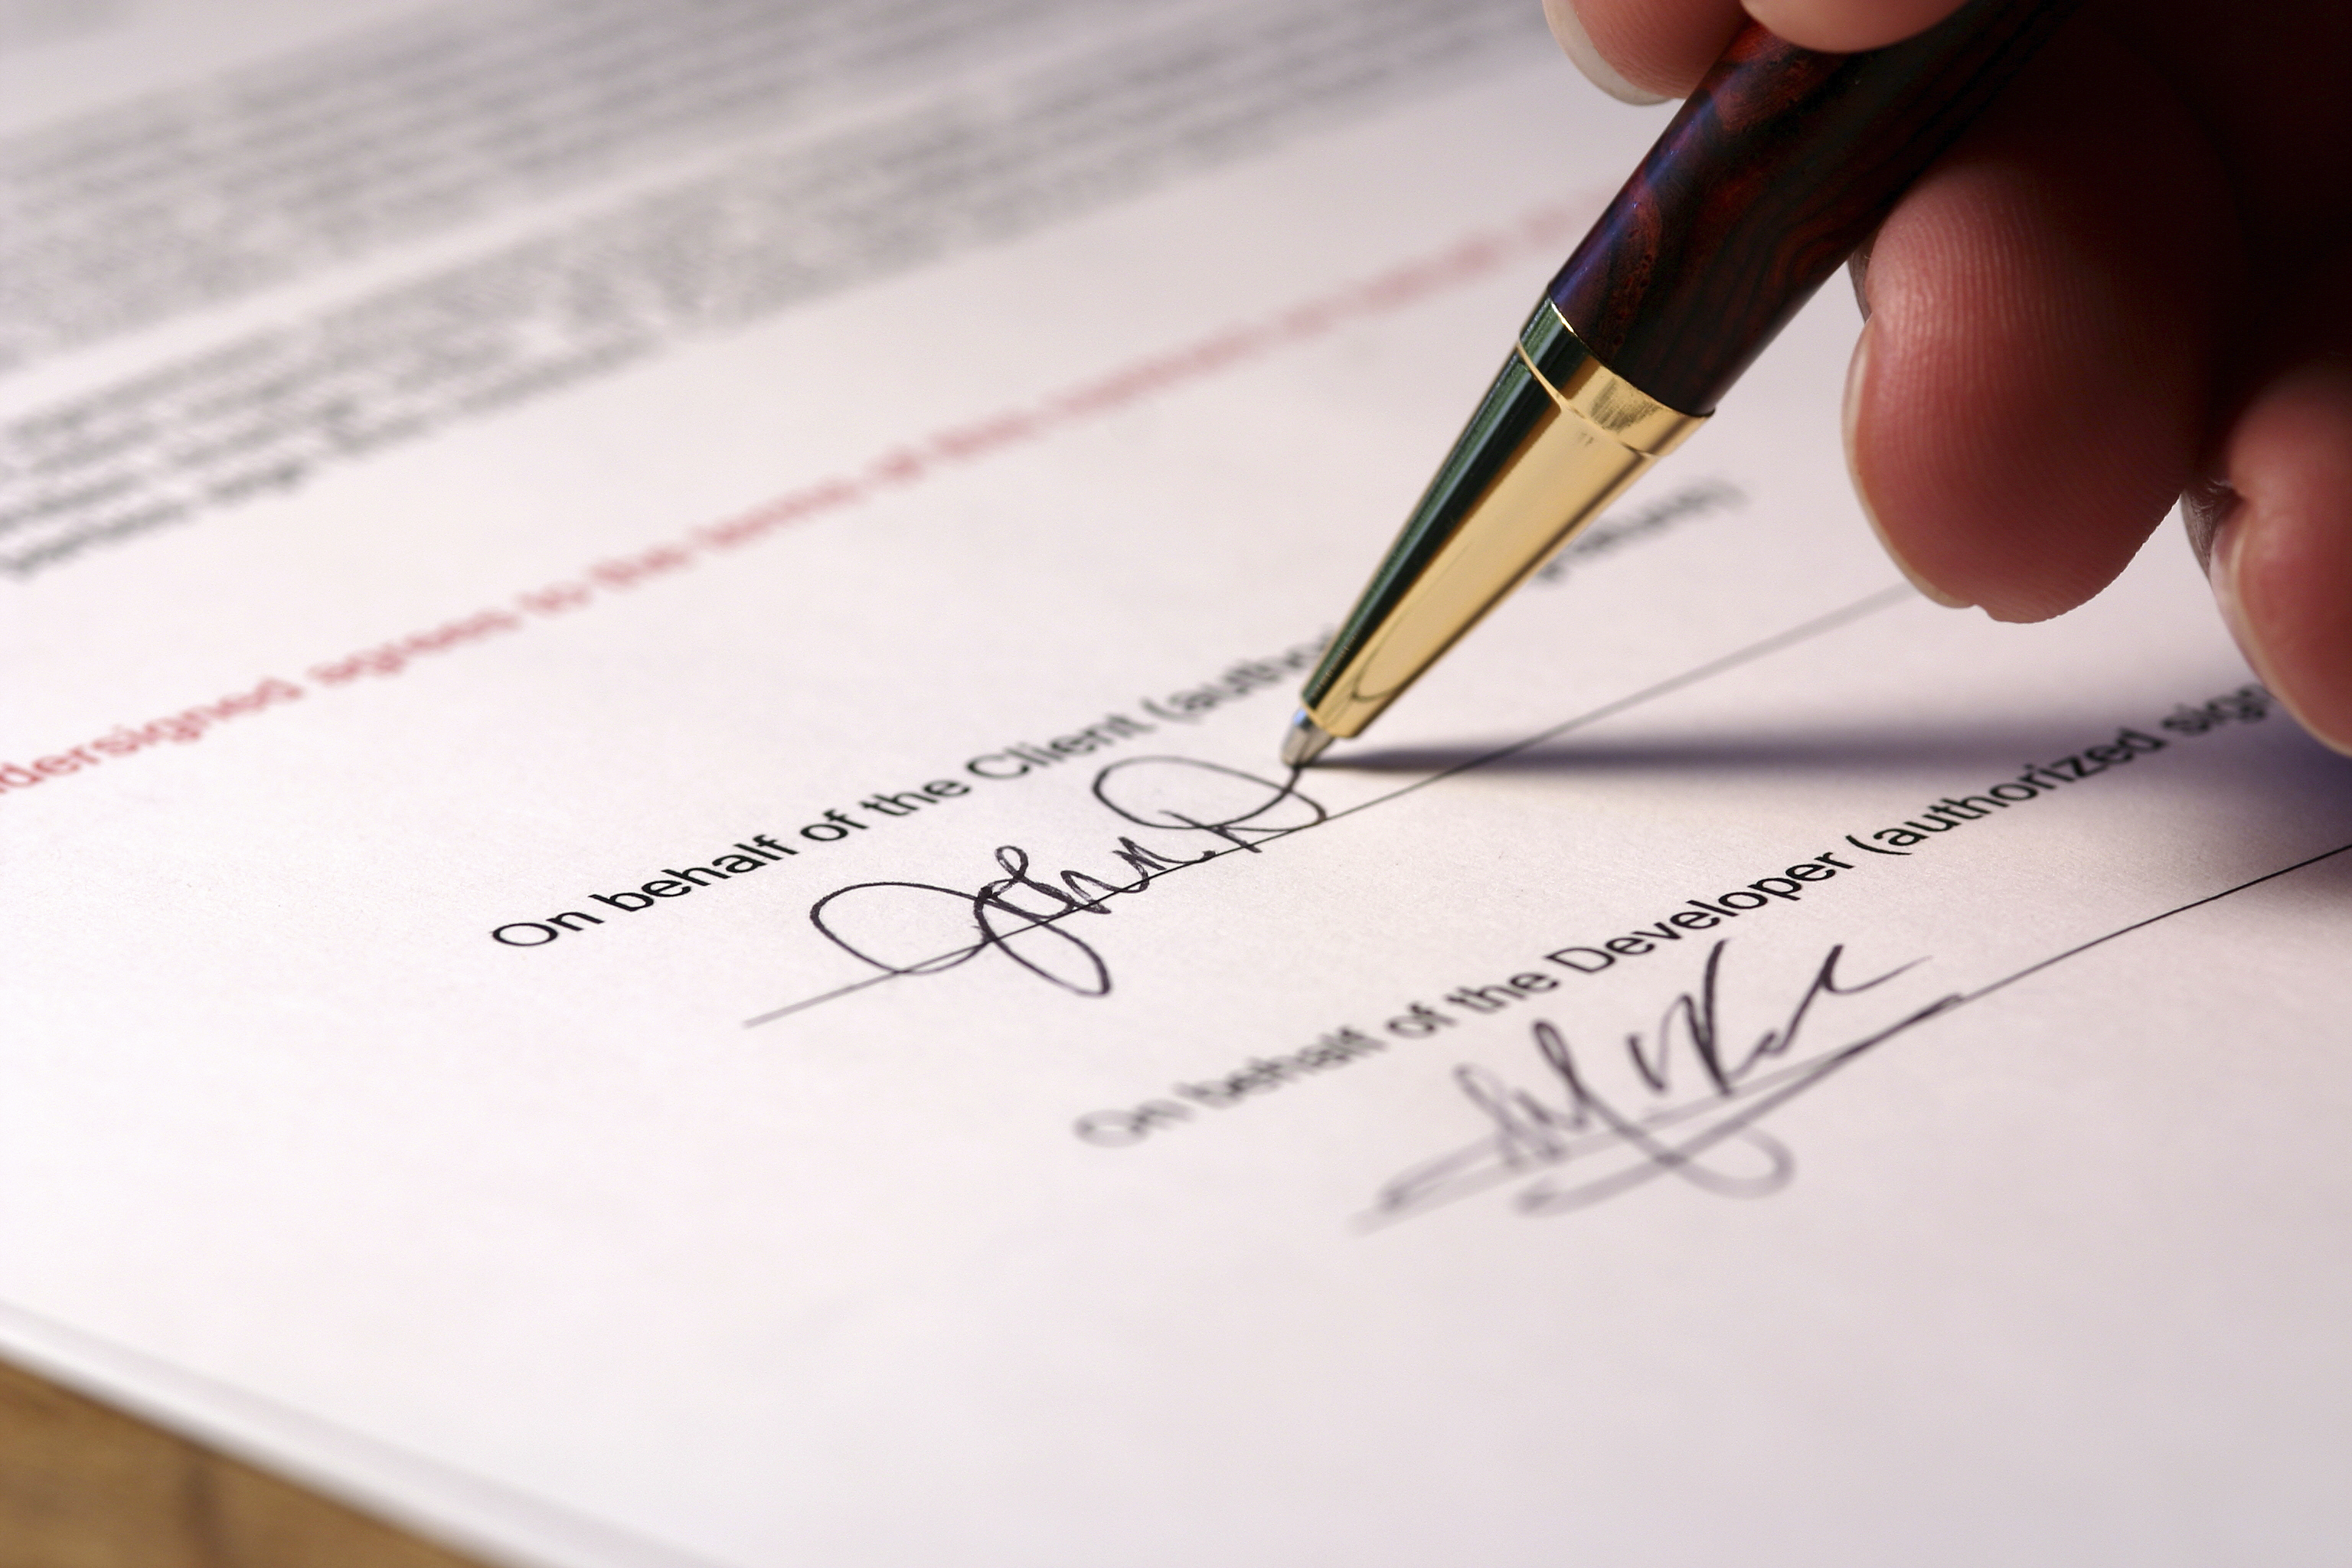
\includegraphics[width=0.32\textwidth]{slides/signing1}} 
\hspace*{0.1in} % separation between the subfigures
 \subfloat{\includegraphics[width=0.32\textwidth]{slides/sigbiometry}} 
\hspace*{0.1in}% separation between the subfigures
\subfloat{\includegraphics[ width=0.3\textwidth]{slides/signing2}} 

  \note{The Handwritten Signature stands as one of the primary methods for identity authentication. This biometric trait can be considered the most legally and socially accepted attributes  for person identification.
  
  \vskip 0.5cm 
  
  In the picture we can see the signature being performedin in a business contract, next using a special kind of digitizing tablet and also on a mobile device, that is an application that is being studied in the field recently.
  }
  
  
\caption{Handwritten Signatures are a widespread biometry.}  %\label{fig:activation}

\end{figure}
\end{frame}




\begin{frame}
\frametitle{Handwritten Signature (2)}

\textbf{The Handwritten Signature widespread can be attributed to \footfullcite{impedovo2008state}:}
\begin{itemize}
\item Signature acquisition is easy and non-invasive;
\item Most individuals are familiar with its use in their daily life;
\item Signatures can be employed as a sign of confirmation in a wide variety of documents, namely, bank checks, identification documents and a variety of business certificates and contracts.
\end{itemize}

 \note{Some of the reasons for handwritten signatures being one of the most widespread biometry, is that \textbf{The Signature acquisition is easy and non-invasive}
 \vskip 0.5cm 
 While most of the biometric identifiers require a special type of device for the identification, handwritten signature based authentication can be performed requiring no sensor except a pen and a piece of paper.
  \vskip 0.5cm 
 Due to its convenient nature, most of individuals are familiar with its use in their daily life
 and Signatures can be employed as a sign of confirmation in a wide set of documents
  \vskip 0.5cm 
 For instance, Bank checks, identification documents and a variety of business certificates and contracts.
 
 \vskip 0.5cm 
  }

\end{frame}

\begin{frame}
\frametitle{Overview of a Handwritten Signature Verification System}
\begin{figure}[!htb]
\centering
\includegraphics[width=\textwidth]{biometry-overview}
\caption{Overview of a typical handwritten signature based system. Figure adapted from \parencite{jain2016} \footfullcite{jain2016}.}
\label{fig_ahsv-overview}
\end{figure}

 \note{\Huge This figure gives an overview of how a signature-based biometric system works.
  \vskip 0.5cm 
  At first, we can see that user \textbf{Y} deposits his \textbf{BIOMETRIC TRAIT} \textbf{B}, in this case a signature, on the system.
  }

\end{frame}

\begin{frame}
\frametitle{Overview of a Handwritten Signature Verification System}
\begin{figure}[!htb]
\centering
\includegraphics[width=\textwidth]{biometryoverview2}

\label{fig_ahsv-overview}
\end{figure}

 \note{\huge If the signature was made on a piece of paper, the signature is inputted to the system using an optical scanner
 \vskip 0.5cm 
   The signatur can also be performed and acquired on a digitzing tablet or a smartphone.
  }

\end{frame}


\begin{frame}
\frametitle{Overview of a Handwritten Signature Verification System}
\begin{figure}[!htb]
\centering
\includegraphics[width=\textwidth]{biometryoverview3}

\label{fig_ahsv-overview}
\end{figure}

 \note{\Huge Next, the system extracts features from the signature sample, represented by the \textbf{X} on the picture.
 
 }

\end{frame}



\begin{frame}
\frametitle{Overview of a Handwritten Signature Verification System}
\begin{figure}[!htb]
\centering
\includegraphics[width=\textwidth]{biometryoverview4}

\label{fig_ahsv-overview}
\end{figure}

 \note{\Huge Then, those features are used to build a database, or a knowledge base, to store the genuine references of the signature of the user.
 
 }


\end{frame}


\begin{frame}
\frametitle{Overview of a Handwritten Signature Verification System}
\begin{figure}[!htb]
\centering
\includegraphics[width=\textwidth]{biometryoverview5}

\label{fig_ahsv-overview}
\end{figure}


 \note{\huge When the system must verify a questioned signature, a score \textbf{S} is obtained according to the similarity of the questioned sample to the reference dataset. The output of the system is either positive (meaning genuien sample)  or negative (meaning a fraud). 
 }
\end{frame}
\begin{frame}
\frametitle{Overview of a Handwritten Signature Verification System}
\textbf{As we can see, a Signature Verification system is essentially a Pattern Recognition application.
}
\vskip 0.5cm
As any Pattern Recognition System, a Signature Verification system has three phases:
\begin{itemize}
\item Data acquisition and preprocessing;
\item Feature extraction;
\item Classification.
\end{itemize}

 \note{\huge As we can see, a Signature Verification system is essentially a Pattern Recognition application.
 \vskip 0.5cm
 As any Pattern Recognition System, a Signature Verification system has three phases: Data acquisition and preprocessing; Feature extraction; Classification.
 
 
 }
 
\end{frame}

\begin{frame}
\frametitle{Online vs Offline Handwritten Signatures}

\begin{figure}[!htpb]
\begin{block}{OFFLINE -> STATIC}
An optical scanner is used to obtain the signature directly from the pen on the paper, and only the digital image of the signature is available.
\end{block}

\begin{block}{ONLINE -> DYNAMIC}
Data is stored during the writing process and consists of a temporal sequence of the three-dimensional coordinates $(x, y, p)$ of consecutive points. 
\end{block}
\centering
 \subfloat[A signature scanned from paper]{\includegraphics[width=0.3\textwidth]{signature.PNG}} 
\hspace*{0.5in} % separation between the subfigures
\subfloat[Digitizing tablet Wacom STU-500] {\includegraphics[width=0.3\textwidth]{stu500.jpg}}
\caption{Different signature acquisition methods. } \label{fig:acquisition}
\end{figure}

 \note{\Large The signature acquisition sensor can be either an optical scanner or an acquisition device such as a digitizing tablet. 
 
  \vskip 0.2cm 
  These two kinds of acquistion methods characterize the two types of signatures: STATIC, offline, AND DYNAMIC, ONLINE
   \vskip 0.3cm 
   In the offline modality, an optical scanner is used to obtain the signature directly from the paper and only a digital image of the signature is available
    \vskip 0.3cm 
    In the online modality, the data is acquired during the signing process and consists of a temporal sequence of the three-dimensional coordinates x, y, p of consecutive points
 }
\end{frame}

\begin{frame}
\frametitle{Online vs Offline Handwritten Signatures (2)}

\begin{figure}[!htpb]

\centering
 \subfloat{\includegraphics[height=0.45\textwidth]{slides/online}} 
\hspace*{0.1in} % separation between the subfigures
\subfloat {\includegraphics[height=0.4\textwidth]{slides/offline}}
\caption{An online and the respective offline signature sample. Extracted from \parencite{galbally2015line} }
\end{figure}
\note{\large In this image, we can see how both modalities are represented
   \vskip 0.5cm 
   The online signature can be thought as a three dimensional time-series, 
   \vskip 0.2cm 
   Meaning that it is the coordinates x, y and pressure over the time.
   
      \vskip 0.5cm 
      While the offline signature is a 2D grayscale (or black and white) digital image.
}
\end{frame}


%\begin{frame}
%\frametitle{Online vs Offline Handwritten Signatures (3)}
%
%
%\begin{block}{ONLINE MODALITY}
%Does not convey information about:
%\begin{itemize}
%\item The overall shape of the signature;
%\item The width of the strokes;
%\item The texture of the ink on the paper.
%\end{itemize}
%\end{block}
%
%
%
%\begin{block}{OFFLINE MODALITY}
%\begin{itemize}
%\item Lost all dynamic information about the signature;
%\item Dynamic features can only be inferred from a static image \parencite{nel2005estimating}. 
%\end{itemize}
%
%\note{\large Specifially, the online modality does not convey information about the shape of the signature, the width of the strokes and the texture of the ink on the paper
%      \vskip 0.5cm 
%Whereas the in the offline modality, the representation has lost all dynamic information about the signature and these dynamic features can only be inferred from a static image.
%}
%
%\end{block}
%
%\end{frame}

\begin{frame}
\frametitle{Handwritten Signature Intra-personal variability}
\begin{figure}[!h]
\centering
\includegraphics[width=0.8\textwidth]{superimposed}
\caption{Superimposed genuine signatures of the same writer. A high intra-personal variability can be noticed. Extracted from \parencite{hafemann2015offline}. }
\label{fig:intraclass}
\end{figure}

\note{As a behavioral trait, signatures present a high intra-personal variability, that is a high similarity between signatures executed by the same writer.

      \vskip 0.5cm 
      there are a variety of human and social aspects that might affect the way we produce our signatures... it might be influenced by sensor limitations, biological aging effects, user emotional state
            \vskip 0.5cm 
	This variability must be taken into account in the authentication process.
	
	      \vskip 0.5cm 
	      
	      It is one of the most challenging aspects of signature verification.
}

\end{frame}

\begin{frame}
\frametitle{Handwritten Signature Inter-personal variability}
\begin{figure}[!htb]
\centering
\includegraphics[width=\textwidth]{forgeries}
\end{figure}

The first column of signatures are genuine references, the following three samples are questioned signatures \footnote{From left to right, top to bottom (F means Forgery and G means Genuine): FGF FFG GFF}. Signature images extracted from \parencite{mcyt-100}.

\note{
Another challenge faced on signature verification systems is the inter-personal variability... \textbf{The similarity between different writers}. This variability is mainly related to malicious people trying to fraud the identity of signers. 	      	      \textbf{talk about the image}
		      	      
		      	      
		      	      	\vskip 0.3cm 
	Forgeries are usually classified in two types: Random forgeries and Skilled Forgeries...
	
		      	      	      
      \vskip 0.3cm 
    Random forgeries: The forger does not attempt to simulate or trace a genuine signature, he tries to verify the identity of a person using his own signature..

      \vskip 0.3cm On the other hand, a skilled forgery, is made by a forger that tries and practices to imitate as closely as possible the genuine signature model. 

}
\end{frame}


%\begin{frame}
%\frametitle{Types of Forgeries}
%In the field of signature verification, forgeries are usually classified into two types \parencite {impedovo2008state}. 
%\begin{itemize}
%\item The first one is the random forgery which is created in a situation which an impostor who has no information about the person or the shape of the original signature tries to verify the identity of a signer using his signature instead of the signature to be tested. The forger does not attempt to simulate or trace a genuine signature.
%
%\item The second type is the skilled forgery, in which the forger tries and practices imitating as closely as possible the static and dynamic information of the genuine signature model. The forger has access for both the user’s name and signature and tries to reproduce it with a similar intra-class variability.
%\end{itemize}
%\end{frame}

%\begin{frame}{Signature Verification Performance}
%Performance on signature verification systems is measured by:
%\begin{itemize}
%\item Genuine rejected as impostor - False Rejection Rate (FRR)
%\item Forger accepted as genuine - False Acceptance Rate (FAR)
%\end{itemize}
%
%\note{
%On the one hand, a genuine signer may be rejected by the system as a potential impostor. False Rejection Rate
%
%	\vskip 0.5cm 
%	On the other hand, a forger might be able to produce a sample which would be accepted as genuine. False Acceptance Rate
%}
%
%\end{frame}

\begin{frame}
\frametitle{Data in Signature Verification}

\vskip 0.2cm

The amount of samples used for training the signature verification system effects the system's performance. 

\vskip 0.2cm

\textbf{As any Pattern Recognition problem, the bigger the dataset, the better the system's performance.}
\vskip 0.2cm

However, in the signature verification context:
\begin{itemize}
\item The amount of data available for each user is often insufficient in real applications;
\item  During the enrollment phase, users are often required to supply only a few samples of their signatures;
\item Acquisition and distribution of real signatures arise legal and privacy concerns;

\end{itemize}

\vskip 0.5cm
\pause
\centering\textbf{The use of realistic synthetic signatures could be regarded as a good alternative.}
 
 \note{
The amount of samples used for training the signature verification system effects the system's performance. As any Pattern Recognition problem, the bigger the dataset, the better the system's performance.
\vskip 0.2cm
However, in the signature verification context some points have to be considered:
\vskip 0.2cm
\vskip 0.2cmThe amount of data available for each user is often insufficient in real applications;
\vskip 0.2cm During the enrollment phase, users are often required to supply only a few samples of their signatures;
\vskip 0.2cmAcquisition and distribution of real signatures arise legal and privacy concerns;
\vskip 0.2cm Therefore, the use of realistic synthetic signatures could be regarded as a good alternative.
 }
\end{frame}


\begin{frame}
\frametitle{Synthetic Samples}

As a consequence, over the last years, several works on both online and offline signature synthesis have been carried out \parencite{galbally2009synthetic, galbally2012synthetic, ferrer2013synthetic, ferrer2013realistic, diaz2014generation}. 
\vskip 0.5cm
\textbf{If the synthetically generated signatures are similar to real ones, it might enable to enlarge existing datasets thus offering better recognition rates.}


\note{
\huge
As a consequence, over the last years, several works on both online and offline signature synthesis have been carried out. 
\vskip 0.5cm
\textbf{If the synthetically generated signatures are similar to real ones, it might enable to enlarge existing datasets to offer better recognition rates.}

}

\end{frame}

\begin{frame}
\frametitle{Online to Offline}
Specifically, one possible synthethis apporach is the generation of synthetic offline signatures based on online samples. 

\vskip 0.5cm
\textbf{ONLINE SIGNATURE $(x_t,y_t,p_t)$ -> OFFLINE SIGNATURE (2D image)}
\vskip 0.5cm

Among others, this type of synthesis approach presents some practical applications:
\begin{itemize}
  \item generation of synthetic static samples to be fused with the original online signatures in order to improve the performance in an online verification scenario;
  \item enlargement of existing offline signature datasets when complementary online data is available;
  \item development of systems capable of integrating both online and offline samples interchangeably, towards a unified signature biometry \parencite{chapter}.
\end{itemize}

\note{
Specifically, one possible synthethis apporach is the generation of synthetic offline signatures based on online samples. 



Among others, this type of synthesis approach presents some practical applications:
\begin{itemize}
  \item creation of synthetic offline samples to be used as a complement to the original online signature to improve the recognition rate of an online verification system.
  
  \item enlarge existing offline signature datasets when complementar online data is available
  \item it can be used to create a unified signature representation, torward a system that can verify both online and offline samples
\end{itemize}
}

\end{frame}

\begin{frame}
\frametitle{Goal}

\centering\Large\textit{The goal of this work is to design an approach to generate synthetic offline handwriting signatures based on online data. 
This problem is modeled as a supervised machine learning task, through a Deep Convolutional Neural Network.
This approach is evaluated in the context of enlargement of offline signature datasets to improve the offline signature verification systems performance.}



\note{
"The goal of this work is to design an approach to generate synthetic offline handwriting signatures based on online data. 
\vskip 0.5cm
IN CONTRAST TO THE STATE-OF-THE-ART
\vskip 0.5cm

We approach this problem as a supervised machine learning task, through a Deep Convolutional Neural Network.
\vskip 0.5cm
Our proposed model is trained to learn the task ``online to offline conversion''
\vskip 0.5cm
This approach is evaluated in the context of enlargement of offline signature datasets to improve the offline signature verification systems performance.}


\end{frame}

\begin{frame}
\frametitle{Specific Goals}
This statement is developed through the following actions:
\begin{itemize}
\item Creation and training of a Deep Neural Network model able to translate dynamic handwritten information into an offline manuscript;
\item Generation of an offline synthetic dataset based on a publicly available online signature dataset
\item Comparison of the proposed approach’s performance with a state-of-the-art method to evaluate the closeness of synthetic signatures with respect to real signatures. 
\end{itemize}

\note{
We design and train a Deep Neural Network model to \textbf{TRANSLATE} DYNAMIC HANWRITTEN INFORMATION to an STATIC IMAGE.
\vskip 0.5cm
We apply our proposed methhod on a publicly available online signature dataset. We generate an offline synthetic dataset.
\vskip 0.5cm
We evaluate the proposed synthetis approach with respect to real signatures and the state-of-the-art.

}

\end{frame}



\begin{frame}
\frametitle{Contents} % Table of contents slide, comment this block out to remove it
\tableofcontents % Throughout your presentation, if you choose to use \section{} and \subsection{} commands, these will automatically be printed on this slide as an overview of your presentation
\note{
From this introduction, the remainder of this presentation is structured as follows:
\vskip 0.5cm

First we will give a brief description of the state-of-the-art method
\vskip 0.5cm
Then we will give a brief overview of the Neural Networks and Deep Learning field, specifically the architecture we used in our proposed method.
\vskip 0.5cm
Then, we describe our proposed method
\vskip 0.5cm
Next, we describe the evaluation setup used to measure our proposed method performance
\vskip 0.5cm
Then we present the results and finally the conclusion and suggestions for future works
}

\end{frame}
%----------------------------------------------------------------------------------------

\section{Off-line Signature Synthesis Using On-line Samples}
\begin{frame}
\frametitle{Off-line Signature Synthesis Using On-line Samples}
\begin{figure}[!htb]
\centering
\includegraphics[width=\textwidth]{slides/ienhanced}
% where an .eps filename suffix will be assumed under latex, 
% and a .pdf suffix will be assumed for pdflatex; or what has been declared
% via \DeclareGraphicsExtensions.
\caption{Method proposed by \cite{diaz2014generation}}
\end{figure}
\note{
This method was proposed by Diaz, they model \textbf{on to off conversion} as a 2D Gaussian function used to convert both pressure and velocity information to create the synthetic sample. 

\vskip 0.5cm
They also use, what refer to an ink-deposition model to estimate how these informations are translted to ink on a paper.

\vskip 0.5cm
The generated signaures have close performance to the real signatures, but when used to increase the training dataset of a system, those samples struggle to improve the recognition rates.
}
\end{frame}

\begin{frame}
\frametitle{Off-line Signature Synthesis Using On-line Samples}
\begin{figure}[!htb]
\centering
\includegraphics[width=\textwidth]{slides/ienhanced-nn}
% where an .eps filename suffix will be assumed under latex, 
% and a .pdf suffix will be assumed for pdflatex; or what has been declared
% via \DeclareGraphicsExtensions.

\end{figure}
\note{
In contrast to what they proposed, instead of modeling this problem as some specific function, we make the neural network learn how this conversion is made, learning from data.
}
\end{frame}

\section{Neural Networks and Deep Learning}

\begin{frame}
\frametitle{Neural Networks}
\begin{itemize}
\item The Biological Neural Network is an essential part of the human brain.
\item The human brain is a complex, non-linear and parallel ``computer'' consisting of \textbf{millions of connected neurons} \parencite{haykin2009neural}.
\item It was observed that the mammal brain is organized in deep neural networks. The brain seems to process information though multiple stages (hierarchies).
\item The depth of the neural network is characterized by the multiple levels of non-linear operations contained in the net.
\end{itemize}
\note{
The Biological Neural Network is an essential part of the human brain.
\vskip 0.5cm
The human brain is a complex, \textbf{non-linear and parallel ``computer''} composed of \textbf{millions of connected neurons}.
\vskip 0.5cm
It was observed that the mammal brain is organized in deep neural networks. The brain seems to process information though multiple stages, or layers.
\vskip 0.5cm
The depth of the neural network is characterized by the multiple levels of non-linear operations contained in the net.
}
\end{frame}

\begin{frame}
\frametitle{Convolutional Neural Networks (CNN)}
\begin{figure}[!htb]
\centering
\includegraphics[width=\textwidth]{lenet}
\caption{Lenet \parencite{lecun1998gradient} \footfullcite{lecun1998gradient}, a convolutional neural network used for handwriting recognition.}
\label{lenet}
\end{figure}

\note{
One of the most succesful applications of deep learning is the convolutional neural network. The CNN is composed of several layers of trainable filters (convolutional layers) and sub-sampling operations, stacked in an alternating sequence starting from the input image.
}
\end{frame}


\begin{frame}
\frametitle{Fully Convolutional Networks (FCN)}
\begin{figure}[!htb]
\centering
\includegraphics[width=0.85\textwidth]{fcn-arch}
\caption{Fully convolutional networks can efficiently learn to make dense predictions for
per-pixel tasks. Extracted from \parencite{long2015fully} \footfullcite{long2015fully}}
\label{fcn-arch}
\end{figure}


\note{
The FCN, is a CNN modified for dense predictions 

While CNNs are typically built in a sequence of convolutional, subsampling, and fully connected layers.
\vskip 0.5cm

The FCN adds an \textbf{expanding path} built with a \textbf{transposed convolutional layer} to recover spatial information.
\vskip 0.5cm
Unlike a common CNN, which learns a general, nonlinear function that characterizes the input
The FCNs \textbf{learn an end-to-end nonlinear mapping} from one input image to another.

\vskip 0.5cm
It is kind of a pixel-wise prediction, where the label space is also transformed from a scalar unit to a two-dimensional image.
}
\end{frame}


\section{Proposed Method}
\begin{frame}
\frametitle{Outline of the Proposed Method}
\begin{figure}[!htb]
\centering
\includegraphics[width=0.8\textwidth]{method}
% where an .eps filename suffix will be assumed under latex, 
% and a .pdf suffix will be assumed for pdflatex; or what has been declared
% via \DeclareGraphicsExtensions.
\caption{The proposed approach diagram and an example of the synthetic signature generation.}
\label{fig_approach}
\end{figure}

\note{
\Huge
In this image, we can see an outline of how the proposed method works.
The input online signature is interpolated to form an 2d Image to be used as input to the trained neural network and producing a synthetic offline signatures, as we can see int the picture.
}
\end{frame}

\begin{frame}{Training Data}


\begin{figure}[!htb]
\centering
\includegraphics[height=0.82\textheight]{dualonoff}

\caption{Figure extracted from \parencite{galbally2015line}}
\label{fig:dualonoff}
\end{figure}

\note{
In order to acquire the online signature as well as the digital image for the same handwriting signal, some points have to be considered.

\vskip 0.5cm

To acquire the data a form must be placed over a digitizng tablet to be filled with an electronic ink-pen. Then, the dynamic data is captured through the tablet, and the paper form can be scanned to provide the static data. 
\vskip 0.5cm

Thereby, two complementary files are available. One contains the dynamic information, and the other digital image.
}
\end{frame}

\begin{frame}{Training Data}
\begin{itemize}
\item We need both the online version of the manuscript mapped to the respective resulting offline representation.
\item Dual modal signature datasets (BiosecurID, Biomet, MyIdea, Sigcomp2009, Sigma, SigwiComp2013, SigWiComp2015) had not this characteristic satisfied. 
\item Although acquired at the same time, both representations of the signatures do not match if we plot it in a single image.
\end{itemize}


\begin{figure}[!htb]

\centering
\includegraphics[width=0.5\textwidth]{onoff}
% where an .eps filename suffix will be assumed under latex, 
% and a .pdf suffix will be assumed for pdflatex; or what has been declared
% via \DeclareGraphicsExtensions.
\caption{A sample from the BiosecurID dataset. Here we can see that the online signature (interpolated in red) can not be projected on the respective offline version.}
\label{fig:onoff}
\end{figure}

\note{
In order to train our model, we need both the online version of the manuscript mapped to the respective resulting offline representation.
\vskip 0.5cm
The publicly available dual modal signature datasets had not this characteristic satisfied. 
\vskip 0.5cm
Although acquired at the same time, when we try to map it, both representations of the signatures do not match

\vskip 0.5cm 
As we can see, for instance, in this sample of the BiosecurID dataset. 
We can notice that the interpolated online signature can not be projected on the respective offline version.
}
\end{frame}

\begin{frame}{Training Data}
%The dual domain IRONOFF \parencite{viard1999ireste} handwriting dataset was thus used to train our model. Besides acquiring both domains of the handwriting manuscript, the online data is mapped to the same coordinate system of the offline data.
%
%Using this dataset, we make the fair assumption that a handwritten signature is a manuscript. With that in mind, we expect that even if the network was trained on handwriting manuscripts, it would work for online signatures to generate its static version.
%


For this reason, we used the IRONOFF handwritting dataset to train our model. The IRONOFF dataset contains a total\textbf{ of 23000 mapped online and offline manuscript samples}.
\begin{figure}[!htb]

\includegraphics{ironoff-mapped}
% where an .eps filename suffix will be assumed under latex, 
% and a .pdf suffix will be assumed for pdflatex; or what has been declared
% via \DeclareGraphicsExtensions.
\caption{An offline manuscript mapped with the respective online trajectory. Image extracted from \cite{viard1999ireste}.}
\label{fig:ironoff-mapped}
\end{figure}

 Using this dataset, we make the fair assumption that if the neural network can perform the conversion on handwriting text, it would also work on handwritten signatures.


\note{
For this reason, we used the IRONOFF handwritting dataset to train our model. The IRONOFF dataset contains a total\textbf{ of twenty three thousand mapped online and offline manuscript samples}.

\vskip 0.5cm
In this image, we can see an interpolated handwriting sample mapped on the respective static image.

\vskip 0.5cm
Using this dataset, we make the fair assumption that if the neural network can perform the conversion on handwriting text, it would also work on handwritten signatures.
}
\end{frame}




\begin{frame}{Preprocessing}

\begin{itemize}
\item Interpolate the online manuscript using the Bresenham algorithm, each pixel has the pressure information;
\item Resize the samples to 383x150 pixels (maintaining the aspect ratio);
\item Invert the pixels (so that the background corresponds to pixel intensity 0);
\item Normalize the input according to the standard deviation of all pixel intensities.
\end{itemize}
\begin{figure}[!htpb]
\centering
 \subfloat[online input]{\includegraphics[width=2.0in]{input-ironoff}} 
\hspace*{0.5in} % separation between the subfigures
\subfloat[offline ground truth] {\includegraphics[width=2.0in]{gt-ironoff}}

\end{figure}

\note{
During the training of our FCN model, two 2D matrices are needed. The online input and the offline target.
\vskip 0.3cm

In order to craete a 2D representation of the online sample, we interpolate the online manuscript using the Bresenham algorithm, where each pixel is the pressure information
\vskip 0.3cm
We resize the samples to a fixed size, using an appraoch to maintain the aspect ratio
\vskip 0.3cm
we also invert the pixels, so that background is represented by the pixel intesity 0 and we normalize the data according to the standard deviation of all pixel intesities
}
\end{frame}

\begin{frame}{Neural Network Model}


\textbf{The FCN was adopted to learn an end-to-end mapping from the online representation to the static image. }
\vskip 0.06cm
\begin{table}[!htb]
\renewcommand{\arraystretch}{1.3}
\caption{The architecutre is a simplified version of the FCN-VGG \parencite{long2015fully, simonyan2014very} }
\centering
\begin{tabular}{|l|l|}
\hline
\textbf{Layer}        & \textbf{Size} \\ \hline
Convolution           & 16x3x3        \\ \hline
Convolution           & 32x3x3        \\ \hline
Convolution           & 32x3x3        \\ \hline
Convolution           & 64x3x3        \\ \hline
Transposed Convolution & 64x3x3        \\ \hline
Transposed Convolution & 32x3x3        \\ \hline
Transposed Convolution & 32x3x3        \\ \hline
Transposed Convolution & 16x3x3        \\ \hline
\end{tabular}
\label{table:cnn-arch}
\end{table}

\note{
The FCN was adopted to learn an end-to-end mapping from the online representation to the static image
\vskip 0.3cm
In this table, we can see the convlutional operations of the model architecture, this neural network architecture is a simplified version of the FCN-VGG.
}

\end{frame}

\begin{frame}{Specific Details of the Neural Network}

Some specific details of the Neural Network:
\begin{itemize}
\item Leaky Rectified Linear Units (LReLUs) were used as the activation function of all convolutional layers;
\pause
\item The ADAM optimizer was used (default parameters) to minimize the Mean Squared Error (MSE) for 100 epochs;
\pause
\item The learning rate was set to 0.001;
\pause
\item Mini-batches of size 16;
\pause
\item The weights were initialized using the method proposed by \cite{glorot2010understanding};
\pause
\item 22000 samples were used for training and 1000 for validation;
\pause
\item The network was trained using the library Tensorflow and it took around five days to train on a GTX 670 GPU.
\end{itemize}
\note{
Leaky Rectified Linear Units were used as the activation function of all convolutional layers; \textbf{NEXT}

\vskip 0.3cm

 The ADAM optimizer was used (default parameters) to minimize the Mean Squared Error (MSE) for a hundred epochs; \textbf{NEXT}

\vskip 0.3cm

 The learning rate was set to dot o o one; \textbf{NEXT}

\vskip 0.3cm
 Mini-batches of size sixteen; \textbf{NEXT}

\vskip 0.3cm
 The weights were initialized using the method proposed by \cite{glorot2010understanding}; \textbf{NEXT}

\vskip 0.3cm
 twenty two thousand samples were used for training and a thousand for validation; \textbf{NEXT}

\vskip 0.3cm
 The network was trained using the library Tensorflow and it took around five days to train on a GTX six hundred seventy GPU.
}

\end{frame}

\begin{frame}
\frametitle{Training results}
\begin{figure}[!htb]
\centering
\includegraphics[width=0.8\textwidth]{iterations}
% where an .eps filename suffix will be assumed under latex, 
% and a .pdf suffix will be assumed for pdflatex; or what has been declared
% via \DeclareGraphicsExtensions.

\caption{Validation loss versus the iterations.}
\label{fig:trainingMSE}

\end{figure}
\note{
\Huge
This is the loss over the iteration graph, we can see that the loss was varying from dot  o o two to dot o o one, from iteration twenty until the last iteration.
}
\end{frame}

\begin{frame}
\frametitle{Training results}
\begin{figure}[!htpb]
\centering
\subfloat{\includegraphics[scale=0.3]{samples/0}} 
\hspace*{0.4in} % separation between the subfigures
\subfloat{\includegraphics[scale=0.3]{samples/00}}
\\
\subfloat{\includegraphics[scale=0.3]{samples/4}} 
\hspace*{0.4in} % separation between the subfigures
\subfloat{\includegraphics[scale=0.3]{samples/04}}
\\
\subfloat{\includegraphics[scale=0.3]{samples/10}} 
\hspace*{0.4in} % separation between the subfigures
\subfloat{\includegraphics[scale=0.3]{samples/010}}
\\
\subfloat{\includegraphics[scale=0.3]{samples/23}} 
\hspace*{0.4in} % separation between the subfigures
\subfloat{\includegraphics[scale=0.3]{samples/023}}
\\
\addtocounter{subfigure}{-8}
\subfloat{\includegraphics[scale=0.3]{samples/30}}
\hspace*{0.4in} % separation between the subfigures
\subfloat{\includegraphics[scale=0.3]{samples/030}} 


\caption{A not cherry-picked selection of synthetic manuscripts produced using our proposed method (left) alongside the expected output (right).} \label{fig:resultingsamples}
\end{figure}
\note{
\Huge
In this picture we can see the sytnhetic samples created with the network, it is somewhat close to the expected output, but in order to have an objective evalution of the quality of the samples in the context of signature verification we performed a machine-oriented evalution.
}
\end{frame}



\section{Evaluation Setup}

\begin{frame}
\frametitle{Evaluation Setup}
To evaluate the quality of the synthetic signatures
\begin{itemize}
\item We use a state-of-the-art offline signature verification system;
\item We use a dataset containing both online and offline signatures.
\end{itemize}

The synthesis quality is measured by the offline verification system performance. \textbf{The questions raised are:}

\begin{itemize}
  \item is the synthetic signatures system performance similar to the offered by real offline signatures?
  \item is it feasible to increase the number of samples at the enrollment phase with the synthetic signatures generated with our proposed method? 
\end{itemize}

\note{
To evaluate the quality of the synthetic signatures
\vskip 0.5cm
We use a state-of-the-art offline signature verification system;
\vskip 0.5cm
We use a dataset containing both online and offline signatures.
\vskip 0.5cm

The synthesis quality is measured by the offline verification system performance. \textbf{The questions raised are:}
\vskip 0.5cm
is the synthetic signatures system performance similar to the offered by real offline signatures?
\vskip 0.5cm
is it feasible to increase the number of samples at the enrollment phase with the synthetic signatures generated with our proposed method? 
}
\end{frame}

\begin{frame}{Offline signature verification system}
Offline handwritten signature verification system:

\begin{itemize}
\item The features were extracted using the approach proposed by \cite{hafemann2017learning} \footfullcite{hafemann2017learning}. This approach uses ideas from transfer learning and multi-task learning to learn features using a Convolutional Neural Network (CNN).

\item The classifier is a Linear SVM
\end{itemize}

\note{
The system used for the evaluation of the real and synthetic signatures is a Linear SVM classifier and with a state-of-the-art feature extraction approach, proposed by Hafeman, Sabouran and Oliveira.
\vskip 0.5cm

The feature extraction system uses ideas from transfer learning and multi-task learning, in the context of offline signature verification, to learn features using a Convolutional Neural Networks (CNN).
\vskip 0.5cm

}
\end{frame}

\begin{frame}{Database}
The evaluation experiments were carried out on the BiosecurID database \parencite{biosecurid}.
\begin{figure}[!htb]
\centering
\includegraphics[height=0.8\textheight]{slides/dataseteval}
% where an .eps filename suffix will be assumed under latex, 
% and a .pdf suffix will be assumed for pdflatex; or what has been declared
% via \DeclareGraphicsExtensions.

\label{fig:multiandmono}
\end{figure}

\note{

It is an online and offline database publicly available containing signatures of \textbf{one hundred thirty two} subjects. Both versions, online and offline, of the same real signature were acquired at the same time.
\vskip 0.2cm
%\item This characteristic, therefore, makes BiosecurID the ideal benchmark for the experimental evaluation conducted in this wor

 The signatures samples were captured in four different sessions, distributed over four months. Each subject signed four times and forged threesignatures per session. 
\vskip 0.2cm
 Therefore, Each subject has sixteen genuine samples and twelve skilled forgeries.

\vskip 0.2cm
For all experiments we splited the dataset as enrollment and test. The first ninety users are used for enrollment and the last forty two are used as the testing set.
\vskip 0.2cm



in the training phase the verification system requires negative samples, we used the MCYT database as the negative dataset samples. 

We selected twenty five random samples from the MCYT dataset to use as negative reference for each user.
}
\end{frame}




\begin{frame}{Experiments}
We follow the same experiment protocol proposed by \cite{diaz2014generation}. 
Two different experiments are carried out. 

\begin{itemize}
\item Experiment 1 focus on evaluating the synthetic signatures performance in comparison to real signatures
\item Experiment 2 evaluates the feasibility of synthetically increasing the number of samples available in a dataset.
\end{itemize}

\note{

We follow the same evaluation protocol followed by Diaz: Two different experiments: Experiment 1 compares the synthetic signatures performance in comparison to real signatures
\vskip 0.2cm
Experiment 2 evaluates the feasibility of increasing the enrollment dataset using synethci samples.

}
\end{frame}


\begin{frame}{Experiment 1}
We evaluate the offline signature verification system performance using only synthetic samples and using only real samples their recognition rates.
\vskip 0.2cm

\textbf{Each user model is trained with:}
\begin{itemize}
\item 4 genuine signatures
\item 25 random samples from MCYT
\end{itemize}

The score is measured with:
\begin{itemize}
\item For each user the remaining 12 genuine samples are used to measure the genuine score. $90 x 12 = 1080$ genuine scores
\item Random impostor scores are calculated comparing the first sample of each test subject to the enrolled model, leading to $90 x 42 = 3780$ random impostor scores.
\item The skilled impostor scores are calculated with the skilled forgeries samples of the enrolled users (12 per subject), leading to $90 x 12 = 1080$ skilled impostor scores.
\end{itemize}

\note{

We evaluate the offline signature verification system performance using only synthetic samples and using only real samples their recognition rates.

\vskip 0.2cm
For each user, we train a model using four genuine signatures and twenty five random samples from MCYT

\vskip 0.2cm
The genuine score is obtained the remaining genuine samples
\vskip 0.2cm
The skileld forgery score is obtained with all skilled forgeries samples of the user
\vskip 0.2cm
And the random forgery score is obtained using 42 signatures from the test set.
}
\end{frame}



\begin{frame}{Experiment 1}
Two different protocols have been considered to compute the 90 users models: a \textbf{mono-session} approach and a \textbf{multi-session} approach.
\begin{figure}[!htb]
\centering
\includegraphics[height=0.7\textheight]{multi-and-mono}
% where an .eps filename suffix will be assumed under latex, 
% and a .pdf suffix will be assumed for pdflatex; or what has been declared
% via \DeclareGraphicsExtensions.

\label{fig:multiandmono}
\end{figure}

\note{

Two enrollment phases are evaluated

\vskip 0.2cm
The difference is the genuine reference used for training the model

\vskip 0.2cm
In the mono-session enrollment, all the four signatures of the first session is used
\vskip 0.2cm
In the multi-session, one sample of each session is used to create the genuine reference set

}

\end{frame}

\begin{frame}{Experiment 2}
Experiment 2 is designed to assess whether \textbf{synthetically increasing the enrollment dataset leads to a better recognition performance}. Three different enrollment sets are considered in this experiment: 
\begin{itemize}
  \item 4 real samples belonging to the
  first acquisition session
  \item 8 real samples belonging to the first and
  the second sessions
  \item 4 real samples belonging
  to the first session plus 4 synthetic samples belonging
  to the second session.
\end{itemize}

\note{

Experiment 2 is designed to assess if the synthetic signatures can be used to increase the training dataset to improve the recognition rates.
\vskip 0.2cm
Three different enrollment sets are considered
}

\end{frame}

\begin{frame}{Experiment 2 - First Enrollment}
\textbf{4 real samples belonging to the first acquisition session}
\begin{figure}[!htb]
\centering
\includegraphics[height=0.7\textheight]{slides/experiment21}
\end{figure}

\note{

The first enrollment set is built with 4 real sigantures, as we can see in the picture
}
\end{frame}


\begin{frame}{Experiment 2  - Second Enrollment}
\textbf{8 real samples belonging to the first and
  the second sessions}
\begin{figure}[!htb]
\centering
\includegraphics[height=0.7\textheight]{slides/experiment22}
\end{figure}

\note{

The second enrollment set is built with eight real signatures from session one and session 2, we expect that the system's performance improves with this enrollment approach.
}

\end{frame}

\begin{frame}{Experiment 2 - Third Enrollment}
\textbf{4 real samples belonging
  to the first session plus 4 synthetic samples belonging
  to the second session.}
\begin{figure}[!htb]
\centering
\includegraphics[height=0.7\textheight]{slides/experiment23}
\end{figure}


\note{

The third enrollment set, uses four real signatures from the first session and four synthetic signatures from the second session.

Given that using eight real signatures is better than using only 4 real signatures, we expect a similar result to using eight real signatures.
}

\end{frame}

\begin{frame}{Performance Assessment}
The performance is measured as the efficiency of the signature verification system.

The system is quantitatively measured by two rates: 
\begin{itemize}
\item False Rejection Rate (FRR): genuine samples classified as forgeries;
\item False Acceptance Rate (FAR): forgeries classified as genuine.
\end{itemize}

When experimenting on signature verification systems, the trade-off between FRR and FAR must be taken into account. When the \textbf{decision threshold is set to have the FRR equal to the FAR, the Equal Error Rate (EER) }is calculated. In our experiments the EER is reported.



\note{

The performance is measured as the efficiency of the signature verification system.
\vskip 0.5cm

The system is quantitatively measured by two rates: False Rejection Rate and False Acceptance Rate
\vskip 0.5cm
When the \textbf{decision threshold is set to have the FRR equal to the FAR, the Equal Error Rate (EER) }is calculated. In our experiments the EER is reported.

}

\end{frame}



\section{Results}
\begin{frame}{Results}




The goal of the experiments are:
\begin{itemize}
  \item Measure the quality of the synthetic images;
  \item Assess whether using synthetic signatures effects the recognition performance of an offline signature verification system; and
  \item Analyze the feasibility of using real and synthetic signatures
  on the enrollment set.
\end{itemize}

We compare our results with the state-of-the-art method, the approach proposed by Diaz \textit{et al.} \textbf{The reported EER is achieved for both approaches in the same experimental conditions.}

\note{

The goal of the experiments are to measure the quality of the synthetic samples, to assess whether synthetic signatures affects the recognition rates of an offline signature verification system and to analyze the feasibility of increasing the training dataset with synthetic samples

\vskip 0.5cm

We compare our results with the approach proposed by Diaz. The reported EER is achieved for both approaches in the same experimental conditions.
}



\end{frame}

\begin{frame}{Results}

We report the results of three versions of the BiosecurID dataset:
\begin{figure}[!htb]
\centering
\includegraphics[width=0.8\textwidth]{slides/split}
% where an .eps filename suffix will be assumed under latex, 
% and a .pdf suffix will be assumed for pdflatex; or what has been declared
% via \DeclareGraphicsExtensions.


\end{figure}

\note{
Three types of signatures are mentioned
\vskip 0.5cm
real offline signatures, which are the corresponding real offline samples, the ideal synthetic signature should be similar to it;
\vskip 0.5cm
synthetic signatures generated with the method proposed by Diaz \textit{et al.} 

\vskip 0.5cm
synthetic signatures created with our proposed method

}
\end{frame}


\begin{frame}{Experiment 1}
\begin{table}[!htb]
%% increase table row spacing, adjust to taste
\renewcommand{\arraystretch}{1.3}
% if using array.sty, it might be a good idea to tweak the value of
% \extrarowheight as needed to properly center the text within the cells
\caption{EER for real, synthetic samples from Diaz \textit{et al.} \cite{diaz2014generation} and our proposed method synthetic offline signatures, for all the approaches considered under the two possible scenarios (i.e., random and skilled forgeries)}
\label{exp1_results_table}
\centering
%% Some packages, such as MDW tools, offer better commands for making tables
%% than the plain LaTeX2e tabular which is used here.
\begin{tabular}{|l|l|l|l|}
    \hline
    \multicolumn{1}{|c|}{\multirow{2}{*}{\textbf{Mode}}} & \multicolumn{3}{c|}{\textbf{Skilled Forgeries}}          \\ \cline{2-4} 
    \multicolumn{1}{|c|}{}                               & \textbf{Real} & \textbf{Diaz \textit{et al.}} & \textbf{Proposed method} \\ \hline
    \textbf{mono-session}                                & 20.28\%            & 23.19\%            & 18.38\%                       \\ \hline
    \textbf{multi-session}                               & 17.59\%            & 22.27\%            & 16.48\%                       \\ \hline
    \multirow{2}{*}{}                                    & \multicolumn{3}{c|}{\textbf{Random Forgeries}}           \\ \cline{2-4} 
    & \textbf{Real} & \textbf{Diaz \textit{et al.}} & \textbf{Proposed method} \\ \hline
    \textbf{mono-session}                                & 9.07\%            & 10.65\%            & 9.99\%                       \\ \hline
    \textbf{multi-session}                               & 5.60\%            & 10.00\%            & 6.48\%                       \\ \hline
\end{tabular}

\end{table}
\note{
In this table we can see that under the skilled forgeries scenario, our proposed method synthetic signatures yields better recognition rates than both real offline signatures and the state of the art method

\vskip 0.5cm
On the random forgeries test we can see that the recognition rates obtained by the real and both types of synthetic samples are close to each other.

}
\end{frame}



\begin{frame}{Experiment 1 - running 30 times}
\begin{figure}[!htb]
\centering
 \subfloat[mono-session - skilled forgeries]{\includegraphics[width=1in]{boxplot/mono-skilled.png}} 
\hspace*{0.1in} % separation between the subfigures
\subfloat[multi-session - skilled forgeries] {\includegraphics[width=1in]{boxplot/multi-skilled.png}}
\hspace*{0.2in} % separation between the subfigures
\subfloat[mono-session - random forgeries]{\includegraphics[width=1in]{boxplot/mono-random.png}} 
\hspace*{0.1in} % separation between the subfigures
\subfloat[multi-session - random forgeries] {\includegraphics[width=1in]{boxplot/multi-random.png}}
\caption{Boxplot comparison for running 30 times the Experiment 1}
\end{figure}

\note{
We can see that when running the experiments 30 times, the results are consistent with a low dispersion around the mean.


\vskip 0.5cm
We can notice that our proposed method is able to generate synthetic signatures comparable to real signatures.
}

\end{frame}

\begin{frame}{Experiment 2}

\begin{table}[!htb]
    %% increase table row spacing, adjust to taste
    \renewcommand{\arraystretch}{1.3}
    % if using array.sty, it might be a good idea to tweak the value of
    % \extrarowheight as needed to properly center the text within the cells
    \caption{EER for real, synthetic samples from Diaz \textit{et al.} \cite{diaz2014generation} and our proposed method synthetic offline signatures for the Experiment 2 under the two possible scenarios, i.e., random (RF) and skilled forgeries (SF)}
    \label{exp2_results_table}
    \centering
    %% Some packages, such as MDW tools, offer better commands for making tables
    %% than the plain LaTeX2e tabular which is used here.
    \begin{tabular}{|l|l|l|}
        \hline
        \multicolumn{1}{|c|}{\textbf{Genuine Training}} & \multicolumn{1}{c|}{\textbf{SF}} & \textbf{RF} \\ \hline
        \textbf{4 real samples}                                         & 21.55\%                     & 10.26\%                         \\ \hline
        \textbf{4 real + 4 real samples}                       & 19.72\%                      & 7.63\%                        \\ \hline
        \textbf{4 real + 4 synthetic from Diaz \textit{et al.}}                           & 24.19\%                         & 7.72\%                \\ \hline
        \textbf{4 real + 4 synthetic from the Proposed Method}                           & 19.17\%         & 9.74\%                        \\ \hline
    \end{tabular}

\end{table}

\note{
In the first line, we can observe the recognition rates obtained using only 4 real samples.
\vskip 0.5cm
Below it, it is reported the recognition rates using 8 real signatures, and 4 real signatures plus the synthetic signatures created with the method proposed by diaz and our proposed method.

\vskip 0.5cm
Specifically, our proposed method yields a improved recognition rate on the skilled forgery scenario
\vskip 0.5cm
In the random forgery scenario the improvement is not as good as using real signatures, but the recognition rate is better than using only four signatures.
}

\end{frame}


\begin{frame}{Experiment 2 - running 30 times}

\begin{figure}[!htb]
\centering
 \subfloat[mixed enrollment - skilled forgeries]{\includegraphics[height=0.7\textheight]{boxplot/mixed-skilled.png}} 
\hspace*{0.8in} % separation between the subfigures
\subfloat[mixed enrollment - random forgeries] {\includegraphics[height=0.7\textheight]{boxplot/mixed-random.png}}
 \label{fig:boxexp2}
\end{figure}

\note{
When running the experiments thirty times, we can notice that the results have a consistent result around the mean.

It is possible for us to conclude that it is possible to user our proposed system to generate synthetic signatures to increase the enrollment dataset and improve the recognition rate of offlien signature verification systems.
}
\end{frame}



\section{Conclusion and Future Works}
\begin{frame}{Conclusion}
\begin{itemize}
\item A Fully Convolutional Neural Network was proposed to learn an end-to-end mapping from the online to the offline domain;
\item We show that it is possible to model the "online to offline signature conversion" as a learning from data task.
\item We observe that the synthetic offline signatures generated with the proposed method offer a verification performance similar to the one offered by real signatures 
\item We show that the synthetic signatures present high discriminative power when used to increase the enrollment set under the skilled forgeries scenario.
\end{itemize}
\note{
A Fully Convolutional Neural Network was proposed to learn an end-to-end mapping from the online to the offline domain;
We show that it is possible to model the "online to offline signature conversion" as a learning from data task.
\vskip 0.5cm
We observe that the synthetic offline signatures generated with the proposed method offer a verification performance similar to the one offered by real signatures 
\vskip 0.5cm
We show that the synthetic signatures present high discriminative power when used to increase the enrollment set under the skilled forgeries scenario.

}
\end{frame}


\begin{frame}{Future Works}
\begin{itemize}
\item Explore the optimization of the hyper-parameters of the FCN
(such as the number of layers, number of neurons per layer, different architectures)
\item Integrate other dynamic features in addition to the pressure on the input of the neural network, such as the velocity.
\item Design a model to synthesize offline signatures with bigger resolution.

\item Combine real online and synthetically generated offline signatures using the
proposed method, when only the online information is available, towards improved
recognition results on a dynamic signature verifier.

\end{itemize}
\note{

Explore the optimization of the hyper-parameters of the FCN
(such as the number of layers, number of neurons per layer, different architectures)
\vskip 0.5cm
Integrate other dynamic features in addition to the pressure on the input of the neural network, such as the velocity.
\vskip 0.5cm
Design a model to synthesize offline signatures with bigger resolution.
\vskip 0.5cm
Combine real online and synthetically generated offline signatures using the
proposed method, when only the online information is available, towards improved
recognition results on a dynamic signature verifier.


}
\end{frame}
\begin{frame}

\begin{minipage}{1\linewidth}
  \centering


  \begin{tabular}{cc}
	\begin{tabular}{c}
		\includegraphics[width=1.0cm]{imagens/brasao.pdf}
		\hspace{0.2cm}
		\includegraphics[width=2.0cm]{imagens/ecomp.pdf}
	\end{tabular}

    \begin{tabular}{c}
      \textbf{Universidade de Pernambuco - UPE} \\ \textbf{Escola Politécnica de Pernambuco - POLI} \\ \textbf{Mestrado em Engenharia da Computação}
    \end{tabular}
  \end{tabular}
\end{minipage}

\titlepage
 \note{ty
 }
\end{frame}

\end{document}
